\documentclass[aapm,graphicx,superscriptaddress]{revtex4-1}
%\documentclass[aapm,reprint]{revtex4-1}
\usepackage{graphicx}
\usepackage{amsmath}
\usepackage{amssymb}
\usepackage[caption=false]{subfig}
% \usepackage{subcaption}
\usepackage[utf8]{inputenc}
\usepackage{color,soul}
\usepackage{algorithm}
\usepackage{algpseudocode}
\usepackage{lineno}
\usepackage{multirow, makecell}
\usepackage{svg}
\newcommand*\mean[1]{\bar{#1}}
\begin{document}

\linenumbers

% tentative title
\title[Robust MBRT for soft tissue sarcoma]{Robust mixed electron-photon radiation therapy planning for soft tissue sarcoma}

\author{Veng Jean Heng}
\email[]{Corresponding author: veng.heng@mail.mcgill.ca}
\affiliation{Department of Physics \& Medical Physics Unit, McGill University, Montreal}
\author{Monica Serban}
\affiliation{Princess Margaret Cancer Centre \& Department of Radiation Oncology, University of Toronto, Toronto}
\author{Marc-Andr\'{e} Renaud}
\affiliation{Gray Oncology Solutions, Montreal}
\author{Carolyn Freeman}
\affiliation{McGill University Health Centre, Montreal}
\author{Jan Seuntjens}
\affiliation{Princess Margaret Cancer Centre \& Department of Radiation Oncology, University of Toronto, Toronto} 
\affiliation{Department of Medical Biophysics, University of Toronto, Toronto}
\date{\today}

\begin{abstract}
\textbf{Purpose:}
Mixed electron-photon beam radiation therapy (MBRT) is an emerging technique which utilizes both external electron and photon beams. It exploits the steep dose falloff and high surface dose of electrons while maintaining target conformity by leveraging the sharp penumbra of photons. This study investigates the clinical benefits of MBRT for soft tissue sarcoma (STS) patients.\\
\textbf{Methods:}
A retrospective cohort of 21 STS of the lower extremity treated with conventional photon-based VMAT were replanned with MBRT. Both VMAT and MBRT treatments were planned on the Varian TrueBeam linac using the Millenium multi-leaf collimator. No electron applicator, cutout or additional collimating devices was used for electron beams of MBRT plans. MBRT treatment planning was performed on an in-house web-based platform using a robust column generation-based optimizer. MBRT plans consisted of a combination of 6 MV photon apertures and electron apertures from 5 energies (6 to 20 MeV). Although previous MBRT work needed shortened electron SSD to achieve acceptable conformity, electron beams in this study were planned at standard 100 cm SAD.\\
\textbf{Results:}
As part of the original VMAT treatment, bolus was required in 10 of the 21 patients. MBRT plans did not require bolus by virtue of the higher electron entrance dose. CTV coverage was found to be clinically equivalent between plans of either modality. Evaluating the absolute paired difference between doses to organs-at-risk in MBRT and VMAT plans, we observed lower to normal tissue in MBRT plans by 13.5\%$\pm$2.9\%. Similarly, to bone was found to be decreased by 3.8\%$\pm$1.8\% of the bone volume. \\
\textbf{Conclusion:}
For STS with subcutaneous involvement, MBRT offers significant sparing of organs-at-risk without sacrificing target coverage when compared to VMAT. MBRT plans were deliverable on conventional linacs without the use of electron applicators, shortened SSD or bolus. This study shows that MBRT is a logistically appealing technique with clear dosimetric benefits.
\end{abstract}

\pacs{}

\maketitle
%for readability on the PDF
\setlength{\baselineskip}{0.7cm}
\section{Introduction}
Soft tissue sarcoma (STS) is a rare malignant tumor that accounts for under 1\% of the total cancer burden \cite{cancerstats2022}. Although they can affect any site of the body, the majority of STS arise in the extremities with 59\% of sarcomas being diagnosed as localized \cite{seer2022}. The primary treatment for STS of the extremities is surgical resection with negative margins. % citation
Current ASTRO guidelines recommend adjuvant preoperative radiation therapy for patients with increased risk of local recurrence \cite{SALERNO2021339}. Image-guided radiation therapy has allowed for more conformal treatment, leading to lower doses to normal tissue and lower risk of wound complications \cite{OSullivan2013, RTOG0630}. Although ASTRO guidelines recommend against the routine use of tissue-equivalent bolus for most sarcomas, it may be used for cases where the CTV involves skin or subcutaneous tissue that cannot receive adequate dose otherwise \cite{SALERNO2021339}. The use of bolus is however associated with higher risks of skin toxicity \cite{PIGNOL2015157, PAREKH20188, WONG2020462} and the variability in its preparation imply higher uncertainty in planning dose calculations.\\

Significant studies have been performed on the feasibility and potential benefits of modulated electron radiation therapy (MERT), delivered using either adjuvant collimators \cite{Lee2000,Ma2000,Hogstrom2004,Gauer2006,Gauer2008,Al-Yahya2007,Alexander2010,Connell2014} or the photon multi-leaf collimators (pMLC) \cite{Lee2000,DuPlessis2006,Klein2008,Salguero2009,Henzen2014}. By leveraging the limited penetration depth and high surface dose of electron beams, electron-only MERT treatment plans were shown to deliver lower doses to normal tissue than photon-only plans. This however came at the cost of worse target dose homogeneity \cite{Alexander2012, Henzen2014}. Mixed electron-photon beam radiation therapy (MBRT) delivered using existing multileaf collimator is an emerging technique that simultaneously optimizes both external electron and photon beam into a single treatment plan \cite{Palma2012, Miguez2017, Renaud2017, Mueller2017, Mueller2018, Renaud2019, Heath2021}. MBRT has been found to provide superior sparing of normal tissue without sacrificing target coverage \cite{Palma2012, Renaud2017, Mueller2017, Mueller2018}. For tumors with superficial involvement, MBRT offers the possibility of excellent target coverage without the use of bolus. 
The steep depth dose curve of electron beams allow MBRT plans to better spare healthy tissue and organs-at-risk (OAR) at depths beyond the tumor. Electron apertures in MBRT deliveries are collimated using only the existing pMLC. Due to significant electron scatter in air, the penumbra of electron beams collimated with pMLC is known to be wider at larger source-to-surface distance (SSD) \cite{Klein1996, DuPlessis2006}. 
Deliveries of electron apertures in MERT and MBRT plans have therefore so far been thought to require shortened SSD of 70-80 cm \cite{Mueller2018Electron}.
Electrons, being charged particles, are also substantially more sensitive to changes in tissue density. It has been shown that MBRT plans must be robustly optimized to properly account for patient setup and motion uncertainty \cite{Renaud2019}. \\

This study seeks to demonstrate the applicability and benefits of MBRT for STS of the extremity. By performing a retrospective treatment planning study, MBRT is dosimetrically compared to the standard of care: photon-based Volumetric Modulated Arc Therapy (VMAT).

\section{Methods}

\subsection{Patient cohort characteristic}

\begin{figure}
    \centering
    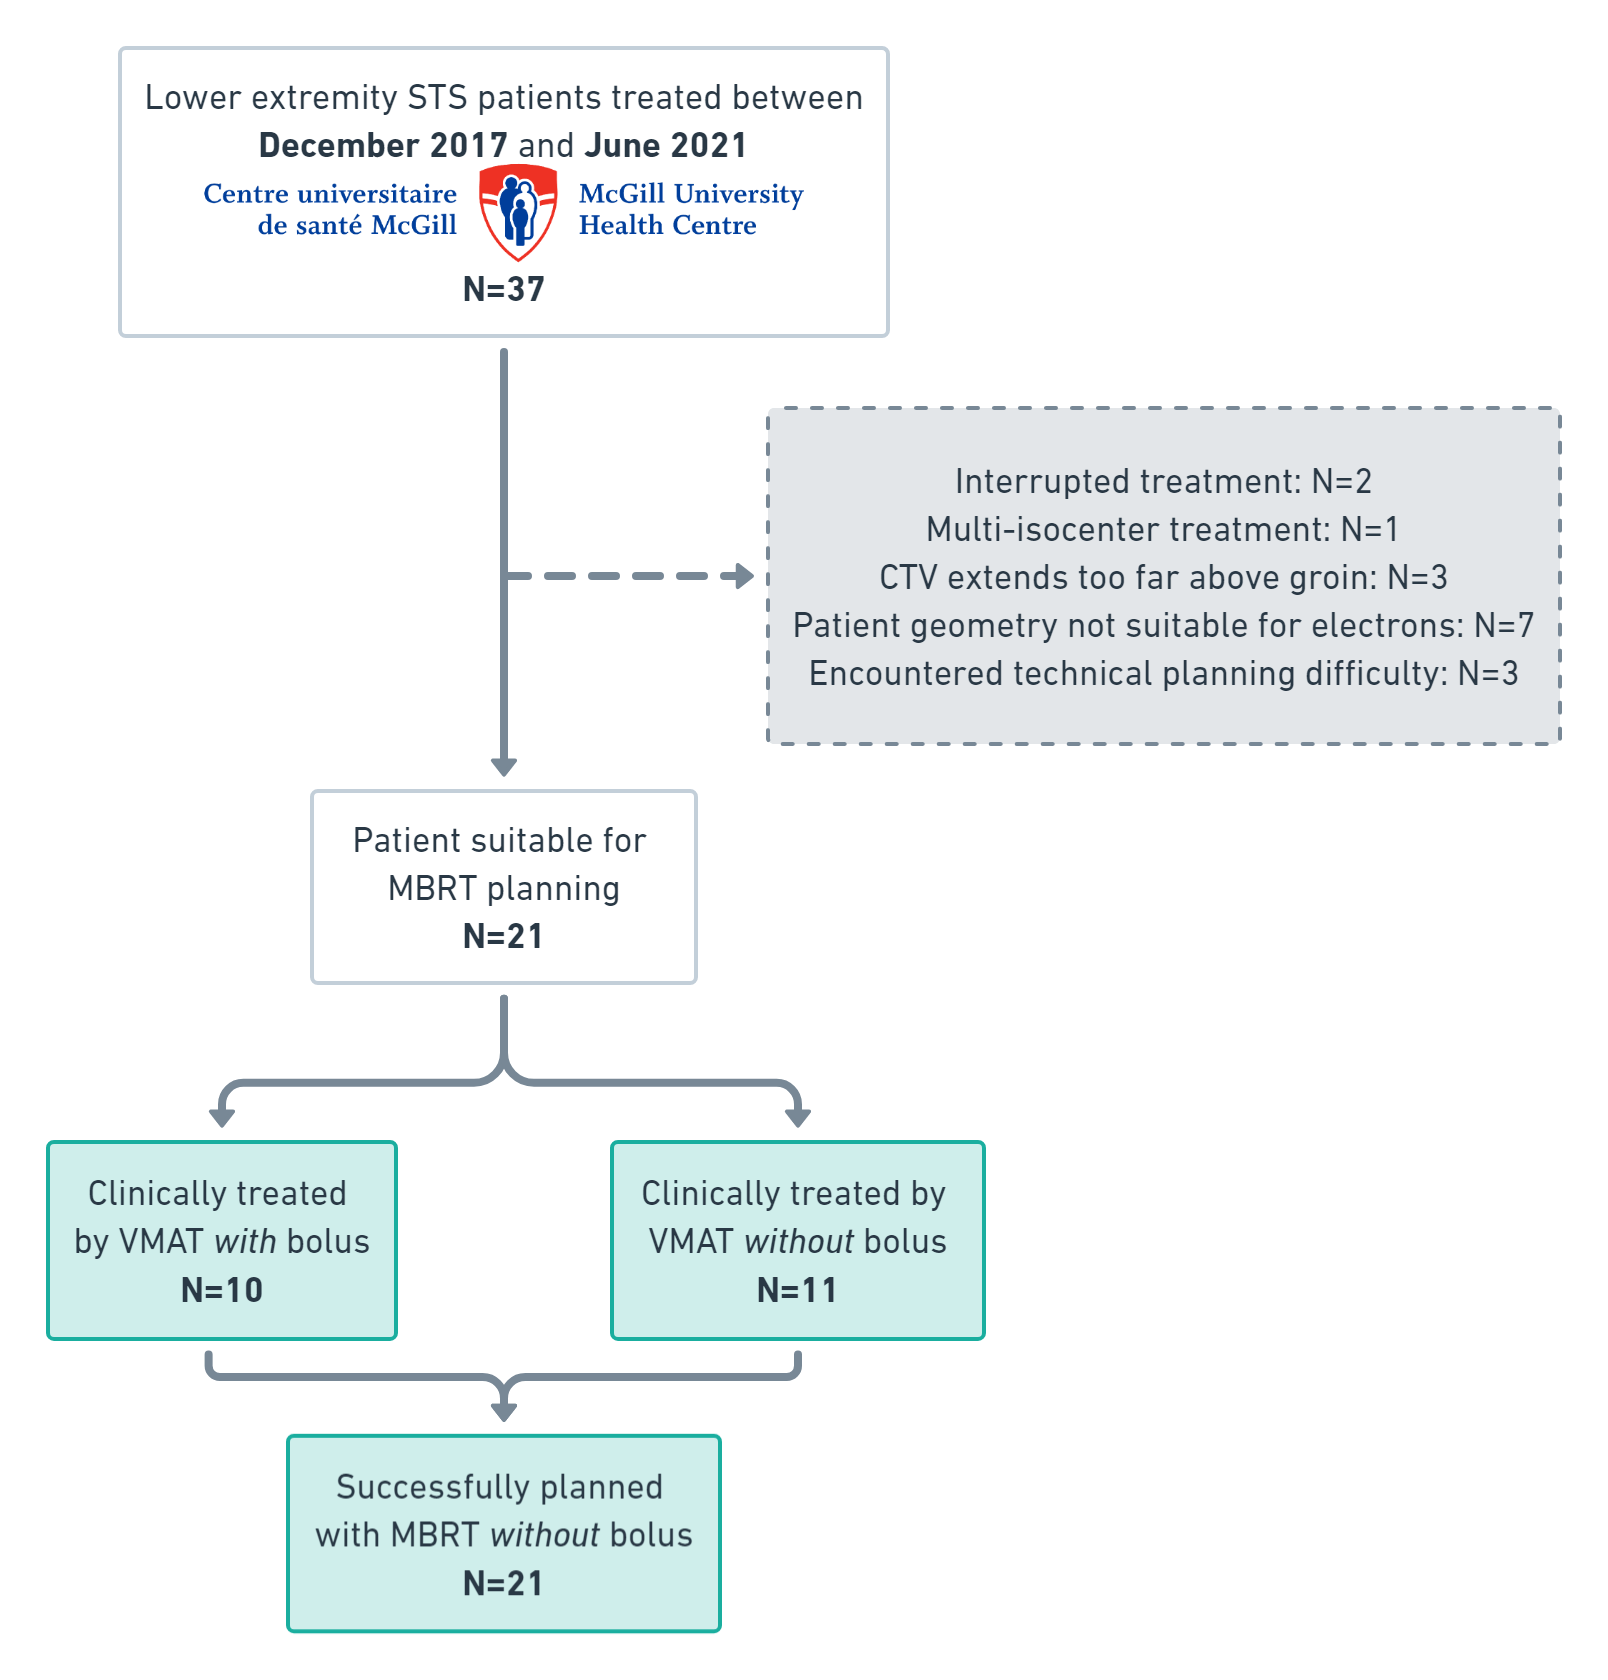
\includegraphics[width=0.7\textwidth]{Consortium diagram.png}
    \caption{Consortium diagram describing patient selection criteria. A total of 37 lower extremity STS patients were found in the time frame Dec. 2017 June 2021. Twenty one patients were finally selected for the planning study. Bolus was not used for any patients in their MBRT plans.}
    \label{fig:consortium}
\end{figure}
A retrospective cohort of STS patients was selected among patients treated at the XXXXX % censored institution name
between December 2017 and June 2021. All patients completed a 25-fraction photon-only VMAT preoperative treatment on a Varian TrueBeam linear accelerator (Varian Medical Systems, Palo
Alto, CA). Only patients with lower extremity STS, without tumor extent above the groin region, were chosen. The consortium diagram (Fig. \ref{fig:consortium}) describes the selection criteria. Planning was performed on a 3 mm slice computed tomography (CT) scan of the patient in the treatment position. Patients were immobilized with a Vac-lok device. Magnetic Resonance Imaging studies were co-registered with CT images to aid the contouring of the gross tumour volume (GTV). For GTVs larger than 8 cm, the clinical target volume (CTV) is contoured with 1.5 cm axial margins and 3 cm cranial-caudal margins from the GTV. For smaller tumours, CTV axial margins of 1 cm and cranial-caudal margins of 2 cm were used. CTV contours did not include any intact bony structures. CTVs are cropped 5 mm from the skin ($n$=8). If full dose to the skin or subcutaneous tissue was required, CTVs were either not cropped when bolus was used (n=10), or cropped to 3 mm when bolus was not used ($n$=3). While following the same skin cropping rule as the CTV, the planning target volume (PTV) consisted of a 5 mm geometrical expansion from the CTV.\\
Contoured OARs relevant for plan optimization included the following: normal tissue strip, bone, femur, joints, anus, skin, testes, and genitalia. The dose constraints to the OAR used during treatment planning are tabulated in Table \ref{tab:OARconstraints}. For consistency, the normal tissue strip OAR was uniformly re-contoured as the subtraction of the PTV and the bone contour from the leg contour, on axial slices within 2 cm proximal and distal to the PTV.\\ 
Treatment planning of VMAT plans were performed on the Eclipse (versions 11 and 15) treatment planning system (TPS). For VMAT plans, a dose of 50 Gy (2 Gy/fraction) was prescribed to 95\% of the PTV. The VMAT plan consisted of either 2 or 3 arcs of 6 MV flattened photon beams delivered at different collimator angles. Only the Varian Millennium MLC was used. Patient doses were calculated with the Analytical Anisotropic Algorithm (AAA). \\

\subsection{MBRT planning}
All patient plans and CT images were exported from Eclipse and imported to an in-house TPS \textit{Brems}. In this study, no MBRT plans made use of bolus. For VMAT plans that required bolus ($n$=10), a new CTV was cropped 2 mm from the skin to allow for buildup. 
For the purpose of MBRT planning, any bolus present in the CT had their density overridden to air. A new skin contour with 2 mm thickness was generated from the patient body contour and was used for both optimization constraints and plan evaluation.\\
MBRT treatments were planned on the same TrueBeam linac originally used for VMAT treatment. For each patient, 3-4 and 5-8 beam angles were selected for the electron and photon components, respectively. Both electron and photon beams were planned as step-and-shoot apertures at standard source-axis distance (SAD) of 100 cm. Both particle types were collimated with the Millennium photon-MLCs. As such, electron fields were planned without the use of standard electron applicators and cutouts.\\
Beamlets were calculated at 5 electron energies (6, 9, 12, 16, and 20 MeV) and at a 6 MV photon beam with flattening filter. Beamlets were robustly calculated to account for positioning uncertainty. This was done by calculating each beamlet in 6 equally weighted additional scenarios, in addition to the nominal (non-shifted) scenario. In each shifted scenario, the isocenter is translated by 5 mm in one of the following directions: $\pm$cranial-caudal, $\pm$anterior-posterior and $\pm$lateral.\\ 
A robust column generation optimizer \cite{Renaud2019} was used to perform simultaneous photon and electron beamlet optimisation of MBRT plans. Optimization constraints were applied on the following structures (if applicable): CTV, contralateral leg, ipsilateral bone, testes, and 2 mm skin. A normal tissue objective (NTO) function was employed to enforce a rapid dose fall-off in voxels outside the CTV. The NTO punishes voxels exceeding a pre-assigned threshold dose. The threshold dose is calculated based on the voxel's distance to the CTV. In general, planning objective weights for each structures were set in the following descending priority order: CTV, skin, NTO, testes, bone, contralateral leg. The plan was normalized such that the average $\mean{V}_{50\text{Gy}}$ over all 7 scenarios of CTV volumes receiving 50 Gy is 95\%. It must be noted that for MBRT plans, robust optimisation is performed on the CTV rather than the traditional PTV-based optimisation.\\
For plan evaluation, patient doses were recalculated in all 7 robust scenarios with an EGSnrc \cite{egsnrc} Monte Carlo model using Varian TrueBeam phase space files. All voxels within the patient body contour were set to water with variable density assigned via a CT-to-mass density curve, exported from Eclipse. As such, dose-to-water is reported in this study. For a fair comparison, the dose of the clinical VMAT plan was also robustly recalculated using the same Monte Carlo model. No renormalization or re-optimization of the VMAT plan was performed at this step.\\

\subsection{Plan evaluation \& statistical analysis}
The Dose-Volume Histogram (DVH) of all patients was computed for the CTV, the ipsilateral bone and the normal tissue strip for each treatment modality. The DVH of the nominal scenario of all 21 plans were aggregated and the mean of each DVH point and its standard error were calculated.\\
For each OAR, the dose metrics tabulated in Table \ref{tab:OARconstraints} were evaluated for both modalities and compared to their corresponding constraints. %In particular, the dose to bone is distinctly different depending on whether the CTV is in contact with the bone contour. Therefore for the evaluation of bone dose, patients were split into 2 groups based on the proximity of their CTV to bone.
In particular, the dose to skin in VMAT plans were found to be distinctly different between patients that required bolus usage and those that did not. As such, for the purpose of the comparison of skin dose, patients were also separated according to their use or non-use of bolus during their VMAT treatment.\\
The dose conformity to the CTV was evaluated using the following definition of the conformity index:
\begin{equation}
    CI = \frac{\text{isodose volume}}{\text{clinical target volume}},
\end{equation}
where the isodose volume corresponds to the sum of volume within the body contour that exceeds a given isodose level. This conformity index was calculated for multiple isodose levels (40\%, 60\%, 80\% and 95\%) to compare the dose fall-off rate of either modality. The homogeneity index was also evaluated on the CTV according to its ICRU83 \cite{ICRU83} definition:
\begin{equation}
    HI = \frac{D2\% - D98\%}{D50\%}.
\end{equation}\\
% The robustness of each modality to setup errors was compared by calculating the CTV's $V_\text{50Gy}$ (100\% of the prescription dose) and $V_\text{47.5Gy}$ (95\% of the prescription dose) in each shift scenario. The distribution of $V_\text{50Gy}$ and $V_\text{47.5Gy}$ were evaluated for the worst-performing scenario of each plan, as well as averaged over all 7 positioning scenarios.

\section{Results}

The mean DVH over the distribution of all 21 patients is plotted in Fig. \ref{fig:dvh_average} for both the MBRT and VMAT plans. The DVH bands represent the $\pm 2 \sigma$ standard error on the mean. Uncertainties on mean values in this study are reported with a coverage factor of $k=2$. MBRT plans provide equivalent CTV DVH as compared to VMAT. The dose to normal tissue and bone, which are the two common OARs in all sarcoma patients, was found to be significantly lower in MBRT plans. For each patient, the DVH of the MBRT plan was subtracted from that of the VMAT plan to show the decrease in dose to OARs in Fig. \ref{fig:dvh_difference_average}. For normal tissue, $V_\text{20Gy}$ was reduced on average by $13.5\%\pm2.9\%$ in MBRT plans. For bone, $V_\text{40Gy}$ decreased by $3.8\%\pm1.8\%$ of the bone volume. The dose constraints for the remaining OARs are evaluated for each plan and plotted in Fig. \ref{fig:oar} as a scatter plot. $V_\text{50Gy}$ to the joint and $D_\text{mean}$ to the femoral head were found to be significantly lower in MBRT plans according to a Wilcoxon signed-ranked test (p=0.002 and p=0.016, respectively). No significant difference was found in the evaluated metric of the other OARs of Fig. \ref{fig:oar}.\\

\begin{figure}[htb]
    \centering
    \includesvg[width=0.8\textwidth]{dvh_average.svg}
    \caption{Aggregate DVH of all 21 patients. Lines represent the mean DVH for each structure and the bands represent the 2 $\sigma$ confidence interval on the mean. The planning constraints for the 2 OARs are plotted as inverted triangles. MBRT plans show equivalent CTV DVH to VMAT with significant reduction in dose to normal tissue and bone.}
    \label{fig:dvh_average}
\end{figure}
\begin{figure}[htb]
    \centering
    \includesvg[width=0.8\textwidth]{dvh_difference_average.svg}
    \caption{Aggregate difference DVH of all 21 patients. Lines represent the mean difference in DVH between the VMAT and the MBRT plan for each patient, while the bands represent the 2 $\sigma$ confidence interval on the mean difference.}
    \label{fig:dvh_difference_average}
\end{figure}
The near-maximum dose $D_\text{0.5cc}$ to a 2 mm thick contour of the skin is plotted in Fig. \ref{fig:skin}. Patients are separated according to their bolus usage in the clinical VMAT plan, while no MBRT plans used bolus. MBRT plans had significantly lower median $D_\text{0.5cc}$ ($50.7\pm0.5$~Gy) than VMAT plans ($52.5\pm0.4$~Gy) in patients that had used bolus. However, in patients that did not use bolus, $D_\text{0.5cc}$ was found to be significantly higher in MBRT plans ($48.4\pm0.5$~Gy) than in VMAT plans ($42.4\pm2.7$~Gy) due to the higher electron surface dose.\\

The conformity index to the CTV was evaluated for 4 isodose levels to compare the rate of the dose fall-off and plotted in Fig. \ref{fig:ctv}. At 95\% of the prescription dose, both the MBRT and VMAT plans for all patients have a CI larger than 1. At the 40\% isodose level (20~Gy), the median CI was found to be significantly smaller in MBRT plans: $2.5\pm0.3$ vs. $3.3\pm0.4$ for VMAT. This indicates a more rapid dose fall-off in MBRT plans outside the CTV, such that a smaller volume of the body is subjected to lower dose baths. \\
The homogeneity index to the CTV is also plotted in Fig. \ref{fig:ctv}. MBRT plans were found to be have a slight but significantly worse (higher) homogeneity index than VMAT plans. This is indicated by a slightly wider CTV DVH curve in MBRT plans as can be seen in the DVHs in Fig. \ref{fig:dvh_average}.\\

A comparison of the two modalities is depicted in Fig. \ref{fig:patient10} for a representative patient of the cohort. A bolus was present for the VMAT treatment of this patient but was overridden to be air for MBRT planning. For the 3 isodose levels that were evaluated (40\%, 80\% and 100\% of the prescription dose), the isodose volume was consistently smaller in the MBRT plan (Fig. \ref{fig:isodose}. This illustrates the steeper dose fall-off that is characteristic to MBRT. Due to this effect, a lower dose to both the normal tissue strip and bone can be observed over almost the entirety of their DVH curves in Fig. \ref{fig:dvh10}. The shaded DVH bands represent the robust range of DVH values as evaluated over 7 positioning scenarios. Without resorting to bolus, the CTV DVH of the MBRT plan can be seen to overlap with the VMAT's DVH, indicating equivalent target coverage. Despite the smaller 50 Gy isodose volume of the MBRT plan, the CTV is adequately covered in all robust scenarios as evidenced by the overlapping CTV bands.

\begin{figure}[htb]
    \centering
    \subfloat[\label{fig:oar}]{
    % \centering
    \includesvg[width=0.71\textwidth]{scatterplot_OAR.svg}
    }
    \subfloat[\label{fig:skin}]{
    % \centering
    \includesvg[width=0.28\textwidth]{boxplot_cropskin_bolus_combined.svg}
    }
    \caption{a) Comparison of the dose to OARs that were not present in all patients. The metric evaluated for each OAR are obtained from Table \ref{tab:OARconstraints}, with $V_{60Gy}$ to the femoral head being 0\% for all plans. The red dotted lines represent the maximum constraint for each metric. b) Near-maximum (0.5 cc) dose to 2 mm skin. The maximum dose constraint to skin (51.5 Gy, 103\% of the prescription dose) is drawn with red dotted lines. Patients are separated according to their bolus usage in their VMAT plans. No bolus was used in any of the MBRT plans.}
\end{figure}
\begin{figure}[htb]
    \centering
    \includesvg[width=0.8\textwidth]{boxplot_ctv_cihi.svg}
    \caption{Left: Conformity index to the CTV for different isodose levels. Right: Homogeneity index to the CTV.}
    \label{fig:ctv}
\end{figure}
\begin{figure}
    \centering
    \subfloat[\label{fig:isodose}]{
    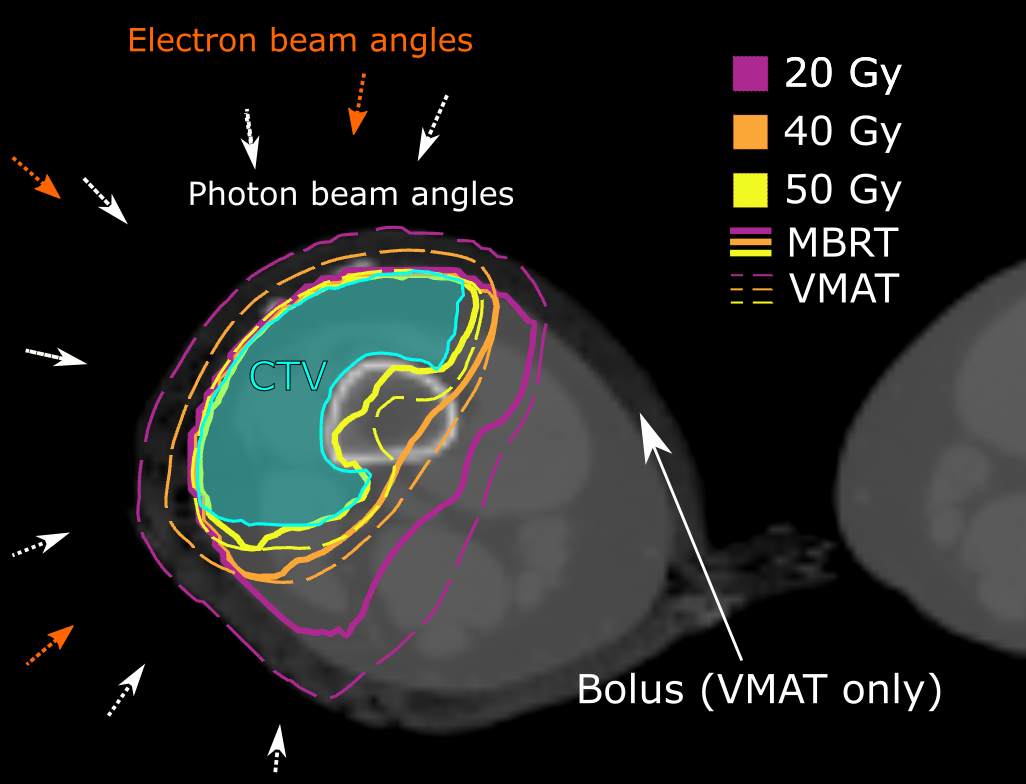
\includegraphics[width=0.56\textwidth]{isodose_cropped.png}}
    \subfloat[\label{fig:dvh10}]{
    \includesvg[width=0.44\textwidth]{dvh_robust_10.svg}}
    \caption{a) Comparison of 3 isodose levels between MBRT (full lines) and VMAT (dashed lines) plans for a representative patient. The MBRT plan can be observed to have a more rapid dose fall-off outside the CTV. The angles of electron (orange) and photon (white) beams in the MBRT plan are illustrated as arrows. The bolus visible in the CT image is only taken into account in the calculation of the VMAT plan; it is overridden to be air for MBRT calculations. b) Comparison of the DVH of the MBRT (full lines) and VMAT (dashed lines) plans for the same patient. The shaded bands represent the range of DVH values attained over 7 positioning scenarios.}
    \label{fig:patient10}
\end{figure}
\section{Discussion}

\subsection{Dosimetric benefit of MBRT for STS}

The average DVH difference plot in Fig. \ref{fig:dvh_difference_average} show consistently lower dose volumes at practically all dose points to the normal tissue contour and bone. The normal tissue was systematically re-contoured to be the subtraction of the PTV and bone contours from the limb contour. Therefore, this result indicates that on average, MBRT plans deliver significantly less dose to voxels outside the target. This effect is even more pronounced when examining volumes subjected to low dose baths. The dose of electron beams falls off much more rapidly with depth than photon beams, and therefore subject fewer voxels beyond the target to low dose baths.\\

The dose to the CTV was found to be slightly less homogeneous in MBRT plans as indicated by the HI in Fig. \ref{fig:ctv}. As MLC-collimated electron beams at SSD 100~cm have inherently wider penumbras than photon beams and a distinct depth dose curve, their usage tends to increase the dose heterogeneity within the CTV. MBRT as a technique aims to compensate for this downside by using both electrons and photons. More electron usage tends to decrease doses beyond the target at the cost of target homogeneity. This is an optimization problem that is defined by the constraints and weights chosen by the planner. During the planning of MBRT plans in this study, a higher importance was placed on obtaining similar target homogeneity as achieved in the clinical VMAT plan. However, higher tissue sparing could be achieved by the optimizer if worse target homogeneity (i.e. hotter spots in the CTV) would be deemed acceptable.

When compared to VMAT plans that used bolus, MBRT plans were found to have lower near-maximum dose to skin. However, when bolus was not used with VMAT, a significantly higher dose to skin was observed with MBRT. This is expected as electron beams have higher entrance doses than photon beams. In this study, the near-maximum dose to skin in MBRT plans were ensured to be lower than 103\% of the prescription dose. This was done by placing an upper optimization constraint on a 2 mm skin contour. As higher weighting is placed on achieving lower doses to skin, the optimizer will tend to reduce the proportion of electrons vs. photons in the MBRT plan. Although reducing electron usage does decrease doses to skin, it also has the effect of increasing dose to deeper normal tissue due to the resulting increase in photons. The planner must therefore make a trade-off between skin dose and normal tissue dose.

\subsection{Logistical benefit of MBRT}

Of the 21 patients that were planned in this study, 10 patients required the use of bolus for their original VMAT treatment. In contrast, no patients required the use of bolus in MBRT plans. Bolus usage entails significant logistical effort in the clinical workflow. Bolus must be positioned in similar conditions during simulation and at every fraction of the treatment. It is difficult to quantify the difference in bolus thickness and density at each instance. This introduces a substantial uncertainty on the dose to the skin and to the target in the VMAT delivery. In addition, bolus usage tends to increase the dose to skin as can be seen in Fig. \ref{fig:skin}, which can lead to acute skin toxicity \cite{PIGNOL2015157, PAREKH20188, WONG2020462}. 

\subsection{Dose-to-water vs. dose-to-medium}
In current clinical practice, dose prescriptions for STS are given as dose-to-water. %citation needed 
As such, all doses in this study have been calculated as dose-to-water to provide a fair comparison. One can wonder if the conclusions of this study would remain true if the absorbed dose-to-medium were to be reported. This is a reasonable concern as electrons are used as part of MBRT plans. Reynaert et al. \cite{REYNAERT201826} have reported that in equilibrium condition, the conversion from dose-to-water to dose-to-bone for photon beams can be approximated by using the ratio of mass energy absorption coefficients. However, the conversion from dose-to-water to dose-to-medium for electrons is dictated by their mass collision stopping power ratio. Therefore, in media where there is a substantial discrepancy between the mass collision stopping power ratio and the mass energy absorption coefficient ratio of medium to water, the conversion to dose-to-medium could differently impact the plan quality of MBRT vs. VMAT plans. The mass collision stopping power ratio of cortical bone (ICRP) to water $[S_\text{col}]^\text{bone}_\text{water}$ for a 12~MeV electron and the mass energy absorption coefficient ratio of cortical bone to water $[\mu_\text{en}]^\text{bone}_\text{water}$ for a 2~MeV photon (most common energy of a 6~MV linac spectrum) can be evaluated, using ESTAR \cite{estar} and XCOM \cite{xcom}, to be:
\begin{equation}
    [S_\text{col}]^\text{bone}_\text{water}(12~\text{MeV}) = \frac{1.819 \text{ MeV cm}^2/\text{g}}{1.989 \text{ MeV cm}^2/\text{g}} = 0.915,
\end{equation}
\begin{equation}
    [\mu_\text{en}]^\text{bone}_\text{water}(2~\text{MeV}) = \frac{2.421 \cdot 10^{-2}\text{ cm}^2\text{/g}}{2.609 \cdot 10^{-2}\text{ cm}^2\text{/g}} = 0.928.
\end{equation}
It must be noted that while electron energy varies with depth, the ratio of stopping power $[S_\text{col}]^\text{bone}_\text{water}$ is mostly constant with electron energy at the relevant energy range and can be arbitrarily evaluated at 12 MeV for the purpose of this argument. Therefore as a very rough approximation, we would expect the conversion of dose-to-water to dose-to-bone to decrease the dose due to 12~MeV electrons by $1-[S_\text{col}]^\text{bone}_\text{water}(12~\text{MeV})/[\mu_\text{en}]^\text{bone}_\text{water}(2~\text{MeV})$ = 1.4\% more than that due to 6 MV photons. However, in practice, the observed difference between MBRT and VMAT plans will be even smaller. This is because electrons only account for a fraction of the patient dose in MBRT plans, with 6 MV photons being responsible for the remaining dose. In addition, as most of the contoured bone volume is cancellous bone with CT number closer to soft tissue, only a fraction of the bone structure would have their medium assigned as cortical bone. The corresponding relative difference in mass collision stopping power ratio and mass energy absorption ratio for soft tissue (ICRP) to water can be calculated to be -0.4\%.\\

To better illustrate this exercise, a patient with significant dose to bone in both the MBRT and VMAT plan was recalculated to score dose-to-medium in medium. The dose ratio as scored to bone vs. water $D^\text{bone}_\text{water}$ was evaluated for all voxels within the bone contour, receiving at least 10 Gy. The average ratio for each modality was found to be:
\begin{equation}
    D^\text{bone}_\text{water}(\text{VMAT}) = 0.9694, D^\text{bone}_\text{water}(\text{MBRT}) = 0.9660,
\end{equation}
such that $1-D^\text{bone}_\text{water}(\text{MBRT})/D^\text{bone}_\text{water}(\text{VMAT})$ = 0.35\%. As this difference is clinically insignificant, the conclusions of this study would therefore not change by scoring dose-to-medium in medium rather than dose-to-water.

\subsection{Contouring inconsistency in sarcoma}

Within the RTOG0630 protocol \cite{RTOG0630} and the current study, the dose to a longitudinal strip of normal tissue is constrained such that $V_\text{20Gy} < 50\%$. However there is no standard definition of the contouring of the normal tissue strip. Depending on the proximity of the normal tissue contour to the CTV and its extent, there is significant variance of the $V_\text{20Gy}$ metric for a same plan. To avoid this inconsistency from introducing bias in the comparison of MBRT and VMAT plans, we have decided to re-contour all normal tissue strips according to a consistent rule described in the \textit{Methods} section. This contouring definition was only applied for the purpose of the dosimetric analysis of the present study and does not constitute a clinical contouring recommendation. In practice, evaluating DVHs on the re-contoured normal tissue has decreased the magnitude in improvements of dose sparing achieved by MBRT plans compared to the original contour. As electrons have wider penumbras, MBRT plans tend to have higher dose in the longitudinal regions immediately outside the CTV. This effect is however compensated by significantly lower doses at depths beyond the CTV. The original tissue strip for patients in our cohort were often contoured to be a thin strip, at the axially opposite edge of the limb (see \textit{Supplementary Material}). Therefore, the dose to this original contour would have been substantially more decreased with MBRT plans as it does not encompass the penumbra regions around the CTV. Nevertheless, despite the more conservative re-contouring rule, lower doses to the normal tissue strip were still observed with MBRT as compared to VMAT. 

% will add a supplementary material figure depicting the new normal tissue contour vs original

\section{Conclusion}

The purpose of this study was to investigate the clinical benefits of MBRT when applied to cases of STS of the extremity. Towards this end, a retrospective MBRT treatment planning study was performed and the resulting plans were compared to the clinically delivered VMAT plans. Without using bolus, MBRT plans achieved clinically equivalent target coverage and homogeneity as compared to VMAT. For all patients, MBRT plans had either significantly lower or equivalent doses to normal tissue and bone. When compared to VMAT plans that did not use bolus, MBRT plans however featured higher dose to skin. On the other hand, For patients that had used bolus, MBRT offers reduction in doses to OARs with no clinically relevant downside. Being deliverable on current state-of-the-art linacs without the use of electron applicators or shortened SSD, MBRT offers its dosimetric benefits at no additional logistical cost. 

\section{Conflict of Interest Statement}
The authors have no relevant conflicts of interest to disclose.

\section{Data Availability Statement}
The data that support the findings of this study are available from the corresponding author upon reasonable request.

\bibliographystyle{ieeetr}
\bibliography{main}

\section{Supplementary material}

\begin{figure}
    \centering
    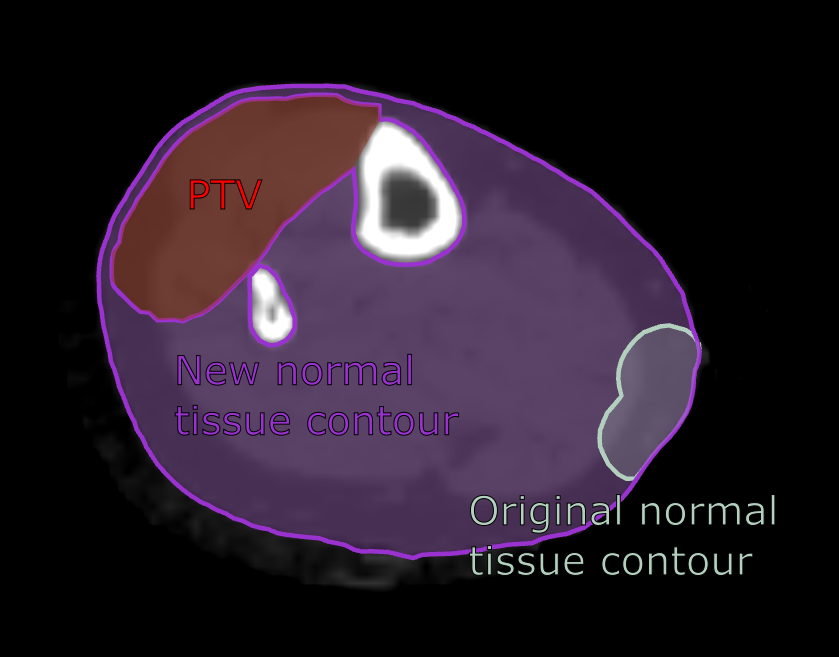
\includegraphics[width=0.7\textwidth]{normaltissue.png}
    \caption{Illustration of the difference between the new normal tissue contour (purple) used in this study and the original normal tissue contour (green) present in the clinical plan. The new contour includes the entirety of the limb excluding PTV (red) and bone, and limited to axial slices within 2 cm proximal and distal to the PTV. The original contour only featured a thin strip that was inconsistently contoured across patients. Comparing MBRT and VMAT doses to the original normal tissue contour would have resulted in even lower doses in MBRT plans than as observed in the new contour.}
    \label{fig:normaltissuecontour}
\end{figure}
\end{document}
